\appendix \label{appendix}
The mapping of the physics tendencies from the physics grid to the GLL grid is done with tensor-cubic Lagrange interpolation. 

The coordinate used for the interpolation is a non-dimensional reference coordinate $(\xi^1,\xi^2)\in [-1:1]^2$ also used internally in the SE dynamical \citep[see, e.g., section 3.3 in ][]{LetAl2017MWR}. The elements of the cubed-sphere in SE are created from an equi-angular gnomonic projection. Consider one element $(\alpha,\beta) \in \left( \alpha^{(elem)}_1,\alpha^{(elem)}_2 \right)\times \left( \beta^{(elem)}_1,\beta^{(elem)}_2\right)$ where $(\alpha,\beta)$ are central angle coordiantes. Let $\Delta \alpha^{(elem)}=\alpha^{(elem)}_2-\alpha^{(elem)}_1$ and $\Delta \beta^{(elem)}=\beta^{(elem)}_2-\beta^{(elem)}_1$. The physics grid cell central angle centers are located at
\begin{equation}
(\alpha^{(phys)}_i,\beta^{(phys)}_j)= \left[ \alpha^{(elem)}_1+\left(i-\tfrac{1}{2}\right) \Delta \alpha^{(phys)},\beta^{(elem)}_1+\left(i-\tfrac{1}{2}\right) \Delta \beta^{(phys)}\right],
\end{equation}
where $\Delta \alpha^{(phys)}=\Delta \beta^{(phys)}=\frac{\Delta \alpha^{(elem)}}{pg}=\frac{\Delta \beta^{(elem)}}{pg}$. The GLL points are located at {\color{red}{add GLL locations...}}. The interpolation is performed in central-angle coordinates using tensor product cubic interpolation {\color{red}{(maybe cite ECMWF techinal report)}}. For elements located on a cubed-sphere edge or corner the coordinate system for neighboring elements may be on a different panel. To take into account this coordinate change the central angle locations of physics grid cell centers located on other panels are transformed to the coordinate system of the panel the element in question is located on \cite[the transformations are given in, e.g.,  ][]{NTL2005MWRb}. An illustration is given in Figure \ref{fig:mapping} for an element located in the lower left corner of a panel. The element in question is $(\xi,\chi)\in (-1,1)^2$ where, for simplicity, we have transformed the element coordinates into normalized coordinates $(\xi,\chi) = \left( \frac{ 2\left(\alpha^{(phys)}-\alpha^{(elem)}_1\right)}{\Delta \alpha^{(elem)}}-1,\frac{2\left( \beta^{(phys)}-\beta^{(elem)}_1\right)-1}{\Delta \beta^{(elem)}}\right)$



In this coordinate system the center of the physics grid cells are located at 
\begin{equation}
(\xi^1_i,\xi^2_j)=\left[ -1+\left(i-\frac{1}{2}\right) \times \Delta \xi,+\left(j-\frac{1}{2}\right) \times \Delta \xi \right],
\end{equation}

\begin{figure}[t]
\noindent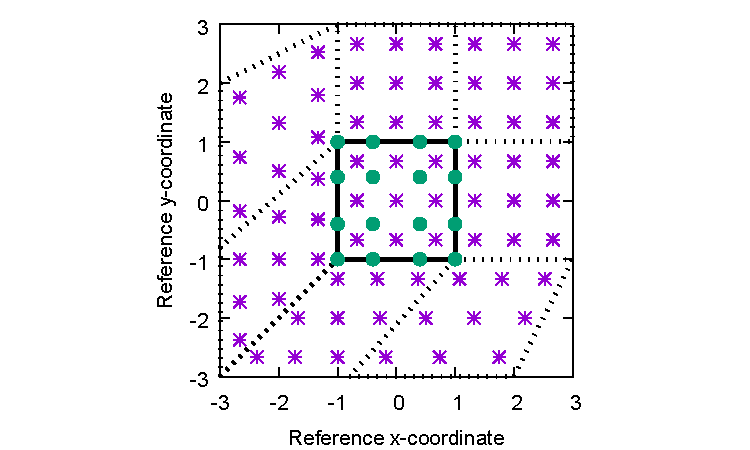
\includegraphics[width=19pc,angle=0]{figs/mapping/mapping.pdf}\\
\caption{}
\label{fig:mapping}
\end{figure}
